\documentclass{beamer}
\usepackage{mathtools,amsthm,bm}
\DeclarePairedDelimiter\ceil{\lceil}{\rceil}
\DeclarePairedDelimiter\floor{\lfloor}{\rfloor}

\usepackage[noend]{algpseudocode}
\usepackage{algorithm}
\newcommand*\Let[2]{\State #1 $\gets$ #2}
\newcommand*{\TO}{\textbf{to}}
% since gemm3 can't be a matro name
\newcommand*{\pluseq}{\mathrel{{+}{=}}}
\newcommand*{\gemmt}{{\textsc{gemm3}}}
\newcommand*{\gemm}{{\textsc{gemm}}}

\usepackage{hyperref}

\usepackage{graphicx}
\usepackage{adjustbox}

\usepackage{tikz}
\usetikzlibrary{matrix,arrows.meta,calc,fit,positioning,chains,shapes}
\definecolor{l3-color}{cmyk}{0,0.06,0.12,0}
\definecolor{l2-color}{cmyk}{0,0.2,0.4,0}
\definecolor{l1-color}{cmyk}{0,0.45,0.55,0}
\definecolor{reg-color}{cmyk}{0.15,0.8,0.8,0}

\tikzset{bpack/.style={to path={
      foreach \i in {1,...,#1} { -- ++(0.5, 0) -- ++ (-0.5,-0.4) } -- (\tikztotarget) \tikztonodes
    }},
  bpack/.default=6,
  apack/.style={to path={
      foreach \i in {1,...,#1} { -- ++(0, -0.5) -- ++(0.4,0.5) } -- (\tikztotarget) \tikztonodes
    }},
  apack/.default=6}

\tikzset{
  label-brace/.style={to path={
      (\tikztostart) ++(#1) -- ++(#1)
      -- ($(\tikztotarget) + 2 *(#1)$) \tikztonodes
      -- +($-1 *(#1)$)
    }},
  brace below/.style={label-brace={0, -3pt}},
  brace above/.style={label-brace={0, 3pt}},
  brace right/.style={label-brace={3pt, 0}},
  brace left/.style={label-brace={-3pt, 0}}}

\tikzset{
  dim-label/.style={label distance=0pt,inner sep=0},
}

\tikzset{
  our-arrow/.style={-{Latex[length=8pt,width=4pt]}},
}

\tikzset{
  memory/.style={fill=white},
  l3/.style={fill=l3-color},
  l2/.style={fill=l2-color},
  l1/.style={fill=l1-color},
  regs/.style={fill=reg-color},
  legend/.style={on chain=labels, minimum height=1ex, minimum width=1em,
    draw, rectangle, outer sep=0, label={[label distance=3pt]right:{\small #1}}}
}

\tikzset{
  loop-label/.style={midway, draw, rectangle},
  square-mat/.style={rectangle,draw,fit={(0, 0) (3, -3)},inner sep=0},
  wide-mat/.style={rectangle,draw,fit={(0, 0) (3, -1)},inner sep=0},
  tall-mat/.style={rectangle,draw,fit={(0, 0) (1, -3)},inner sep=0}
}

\newcommand*{\bpackarr}[2][6]{\draw[our-arrow] ($(#2 - 0.75, -0.25)$) to[bpack=#1] ++($(0.5, -0.4 * #1)$);}
\newcommand*{\apackarr}[2][6]{\draw[our-arrow] ($(0.25, - #2 + 0.75)$) to[apack=#1] ++($(0.4 * #1, -0.5)$);}

\newcommand*{\bracelabel}[4]{\draw (#1) to[brace #3]%
  node[midway,label={[dim-label]#3:#4}] {} (#2);}

\newcommand*{\packlabel}[3]{\path (#1) -- (#2)%
  node[midway,label={#3:pack}] {};}

% [style] name width height N code-for-every
\newcommand*{\vgrids}[6][fill=white]{
  \foreach \x in {1, ..., #5} {
    \node[rectangle, draw, #1,fit={($(#3 * \x - #3, 0)$) ($(#3 * \x, -#4)$)}, inner sep=0] (#2\x) {};
    #6
  }
}
% [style] name width height N code-for-every
\newcommand*{\hgrids}[6][fill=white]{
  \foreach \y in {1, ..., #5} {
    \node[rectangle, draw, #1,fit={($(0, -\y * #4 + #4)$) ($(#3, -\y * #4)$)}, inner sep=0] (#2\y) {};
    #6
  }
}

% [first-style] style name width height N code-for-every
\newcommand*{\vgridscache}[7][memory]{
  \foreach \x in {1, ..., #6} {
    \ifnum\x=1%
    \node[rectangle, draw, #1 ,fit={($(#4 * \x - #4, 0)$) ($(#4 * \x, -#5)$)}, inner sep=0] (#3\x) {};
    \else
    \node[rectangle, draw, #2 ,fit={($(#4 * \x - #4, 0)$) ($(#4 * \x, -#5)$)}, inner sep=0] (#3\x) {};
    \fi
    #7
  }
}
% [first-style] style name width height N code-for-every
\newcommand*{\hgridscache}[7][memory]{
  \foreach \y in {1, ..., #6} {
    \ifnum\y=1%
    \node[rectangle, draw, #1,fit={($(0, -\y * #5 + #5)$) ($(#4, -\y * #5)$)}, inner sep=0] (#3\y) {};
    \else
    \node[rectangle, draw, #2,fit={($(0, -\y * #5 + #5)$) ($(#4, -\y * #5)$)}, inner sep=0] (#3\y) {};
    \fi
    #7
  }
}

\newcommand*{\pluseqnode}[1]{\node[at={(0, -1.5)}] (#1-plus) {\large $\pluseq$};}

% [style] N N - 1 offset-right
\newcommand*{\loopborder}[3][black]{\draw[rounded corners, color=#1]%
  (#2-loop.west) -| ($(#3-rect-west) + (-5pt, -5pt)$) coordinate (#2-rect-west)%
  -- ($(#3-rect-east) + (5pt, -5pt)$) coordinate (#2-rect-east)%
  |- (#2-loop.east);}


\tikzset{
  invisible/.style={opacity=0,text opacity=0},
  visible on/.style={alt={#1{}{invisible}}},
  alt/.code args={<#1>#2#3}{%
    \alt<#1>{\pgfkeysalso{#2}}{\pgfkeysalso{#3}} % \pgfkeysalso doesn't change the path
  },
  explanation/.style={visible on=<2->},
  graph-pic/.style={anchor=north west, at={(0, 0)},inner sep=0pt}
}

\useoutertheme{infolines}
\setbeamertemplate{navigation symbols}{}

\title[\gemmt{}]{\gemmt{}: Constant-workspace high-performance multiplication of three matrices for matrix chaining}
\author[Drewniak]{Krzysztof A. Drewniak}
\institute[UT Austin]{The University of Texas at Austin}
\date[]{April 13, 2018}

\begin{document}
\begin{frame}[plain]
  \titlepage{}
\end{frame}

\section[Introduction]{Introduction}
\begin{frame}
  \frametitle{Matrix chaining problem}
  \begin{itemize}
  \item Problem: compute $A_1A_2\cdots A_n$ efficiently
  \item $O(n \log n)$ algorithm, also $O(n^3)$ with dynamic programming
  \item Fewer flops $\to$ more performance?
  \end{itemize}
\end{frame}

\begin{frame}
  \frametitle{Generalized matrix chaining}
  \begin{itemize}
  \item In reality --- transposes, inverses, properties
  \item
    \begin{description}
    \item[Ensemble Kalman filter] $X_i^b S_i (Y_i^b)^T R_i^{-1}$
    \item[Tridiagonalization] $\tau_u\tau_vvv^TAuu^T$
    \item[Two-sided triangular solve] $L^{-1}AL^{-H}$ ($L$ lower triangular)
    \end{description}
  \item Performance with BLAS/LAPACK -- must be expert
  \item Less performance with  Matlab, numpy, etc. (left-to-right)
  \item Linnea: expression $\to$ BLAS calls automagically
  \end{itemize}
\end{frame}

\begin{frame}
  \frametitle{\gemmt{} --- Why bother?}
  \begin{itemize}
  \item
    \begin{itemize}
    \item $\bm{X_i^b S_i (Y_i^b)^T}R_i^{-1}$
    \item $\tau_u\tau_v \bm{vv^TAuu^T}$
    \item$\bm{L^{-1}A(L^{-1})^H}$ ($L$ lower triangular)
    \end{itemize}
  \item All multiply three matrices as a subproblem
  \item (Notation: $G \pluseq DEF$ and \gemmt{})
  \end{itemize}
\end{frame}

\begin{frame}
  \frametitle{\gemmt{} --- Why a new algorithm?}
  \begin{itemize}
  \item Current approach: parentheses, multiply twice, store temporary $T$
  \item $T$ often eats memory (\& perf)
  \item We can do better!
  \item Use how \gemm{} works to nest computations
  \item $O(1)$ extra memory, maybe more performance
  \end{itemize}
\end{frame}

\section[\gemm{}]{High-Performance \gemm{}}
\frame{\sectionpage}

\begin{frame}
  \frametitle{Memory hierarchy}
  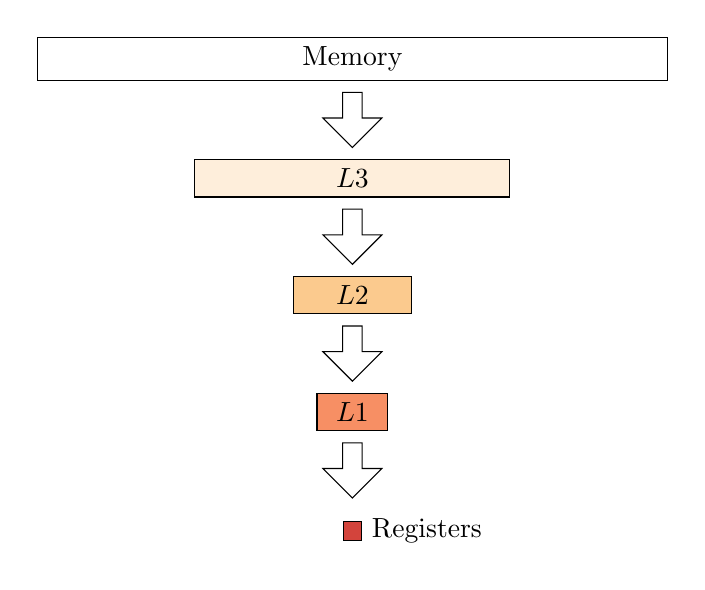
\begin{tikzpicture}[read-point/.style={single arrow,minimum height=0.7cm, minimum width=0.1cm, draw, shape border rotate=270}]
    \matrix [matrix of nodes, nodes={draw}, row sep=4pt] {
      |[memory, minimum width=8cm]| Memory\\
      |[read-point]|\\
      |[l3, minimum width=4cm]| $L3$\\
      |[read-point]|\\
      |[l2, minimum width=1.5cm]| $L2$\\
      |[read-point]|\\
      |[l1, minimum width=0.9cm]| $L1$\\
      |[read-point]|\\
      |[regs, minimum width=0.2cm, label=right:Registers]|\\
    };
  \end{tikzpicture}
\end{frame}

\begin{frame}
  \frametitle{Important matrix shapes}
  \begin{adjustbox}{max size={!}{0.87\textheight},center}
  \begin{tikzpicture}
    \matrix (pics)[column sep=0.2cm, row sep=5.5ex, ampersand replacement=\&] {
      \node[square-mat] {Block};\\
      \node[wide-mat] {Row panel};\\
      \node[tall-mat,label={right:Column panel}] {};\\
    };
  \end{tikzpicture}
  \end{adjustbox}
\end{frame}

\begin{frame}
  \frametitle{\gemm{}: The kernels}
  \begin{adjustbox}{max size={!}{0.87\textheight},center}
  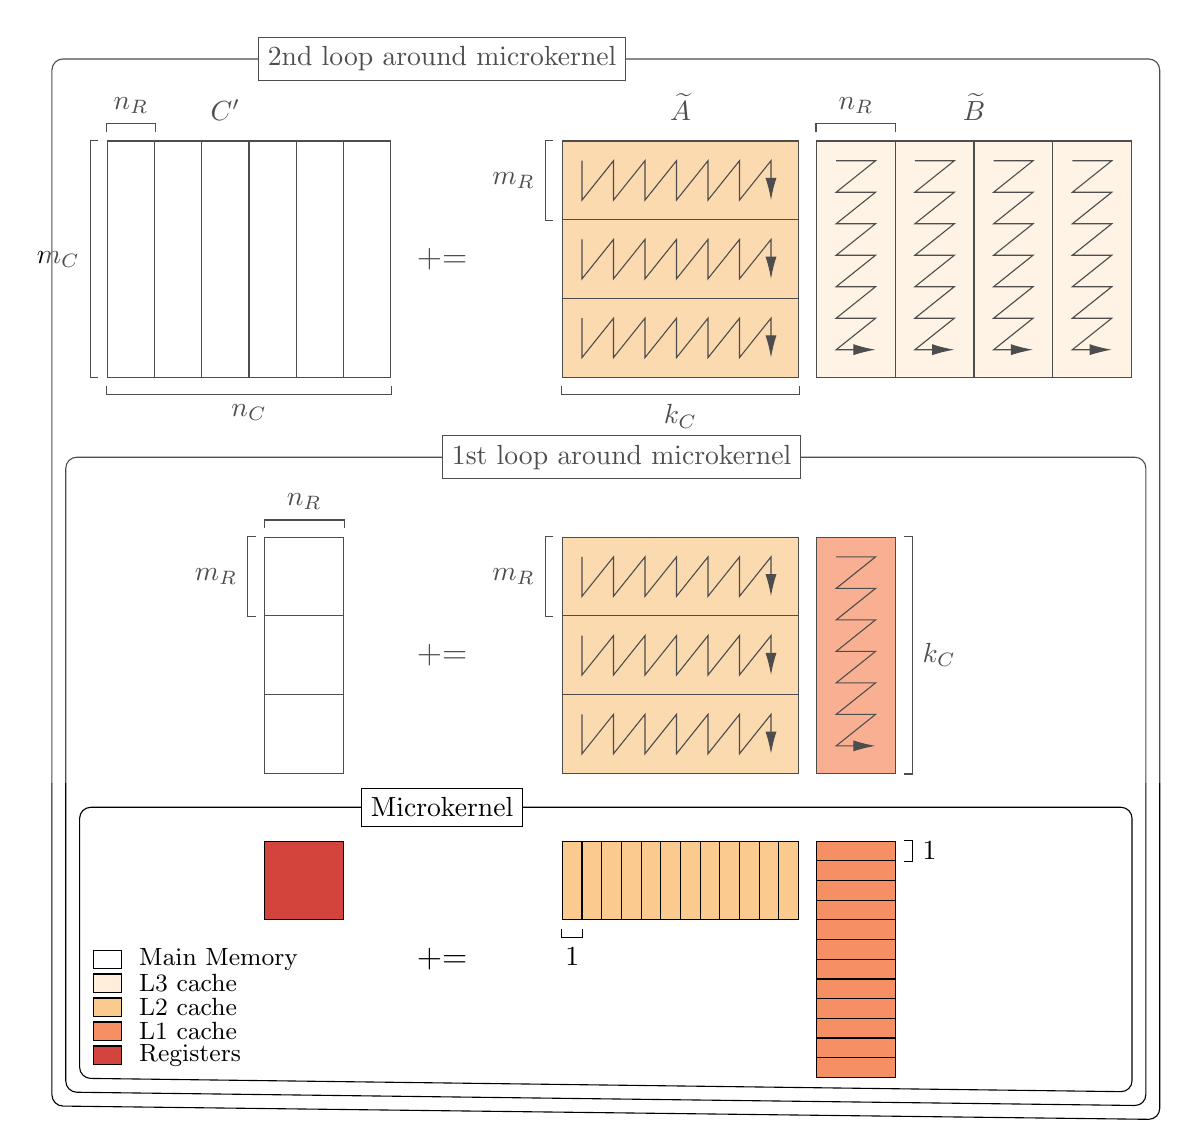
\begin{tikzpicture}
    \matrix (loops)[column sep=0.2cm, row sep=5.5ex] {
  \vgrids[memory]{2C}{0.6}{3}{6}{}
  \bracelabel{2C1.north west}{2C1.north east}{above}{$n_R$}
  \bracelabel{2C1.south west}{2C6.south east}{below}{$n_C$}
  \bracelabel{2C1.north west}{2C1.south west}{left}{$m_C$}
  \path (2C1.north west) -- (2C5.north east) node[midway,label={above:$C'$}] {};&

  \pluseqnode{2}&

  \hgrids[l2]{2A}{3}{1}{3}{\apackarr{\y}}
  \bracelabel{2A1.north west}{2A1.south west}{left}{$m_R$}
  \bracelabel{2A3.south west}{2A3.south east}{below}{$k_C$}
  \path (2A1.north west) -- (2A1.north east) node[midway,label={above:$\widetilde{A}$}] {};&

  \vgrids[l3]{2B}{1}{3}{4}{\bpackarr{\x}}
  \bracelabel{2B1.north west}{2B1.north east}{above}{$n_R$}
  \path (2B1.north west) -- (2B4.north east) node[midway, label={above:$\widetilde{B}$}] {};\\

  \foreach \y in {1,...,3} {
    \node[rectangle, draw, fit={(2, -\y + 1) (3, -\y)}, inner sep=0] (1C\y) {};
  }
  \bracelabel{1C1.north west}{1C1.south west}{left}{$m_R$}
  \bracelabel{1C1.north west}{1C1.north east}{above}{$n_R$}&

  \pluseqnode{1}&

  \hgrids[l2]{1A}{3}{1}{3}{\apackarr{\y}}
  \bracelabel{1A1.north west}{1A1.south west}{left}{$m_R$}&

  \vgrids[l1]{1B}{1}{3}{1}{\bpackarr{\x}}
  \bracelabel{1B1.north east}{1B1.south east}{right}{$k_C$}\\


  \node[rectangle, draw, regs, fit={(2, 0) (3, -1)}, inner sep=0] (0C) {};
  \begin{scoped}[start chain=labels going {below=2pt of \tikzchainprevious}]
    \node[legend=Main Memory, memory] at (0, -1.5) {};
    \node[legend=L3 cache, l3] {};
    \node[legend=L2 cache, l2] {};
    \node[legend=L1 cache, l1] {};
    \node[legend=Registers, regs] {};
  \end{scoped}&

  \pluseqnode{0}&

  \vgrids[l2]{0A}{0.25}{1}{12}{}
  \bracelabel{0A1.south west}{0A1.south east}{below}{$1$}&

  \hgrids[l1]{0B}{1}{0.25}{12}{}
  \bracelabel{0B1.north east}{0B1.south east}{right}{$1$}\\
};
\path node[draw,above=2cm of 2-plus] (2-loop) {2nd loop around microkernel}
(2-plus) -- (1-plus) node[loop-label,anchor=west] (1-loop) {1st loop around microkernel}
(1-plus) -- (0-plus) node[loop-label] (0-loop) {Microkernel};

\draw[rounded corners] let \p1 = ($(0B12.south east) + (0pt, -5pt)$),
\p2 = ($(2B4.south east) + (0pt, -5pt)$),
\p{east} = (\x2, \y1) in
(0-loop.west) -| ($(labels-end.south west) + (-5pt, -5pt)$) coordinate (0-rect-west)
-- (\p{east}) coordinate (0-rect-east)
|- (0-loop.east);

\loopborder{1}{0}
\loopborder{2}{1}

    \path let \p{north} = (2-loop.north),
    \p{west} = (2-rect-west),
    \p{east} = (2-rect-east)
    in node [fit={(\x{west}, \y{north}) (1B1.south east) (\x{east}, \y{north})},
    fill=white, opacity=0.3, visible on=<-1>] (hide-square) {}
    coordinate [visible on=<2->] (dummy-coord);
  \end{tikzpicture}
  \end{adjustbox}
\end{frame}

\begin{frame}
  \frametitle{\gemm{}: The algorithm}
  \begin{adjustbox}{max size={!}{0.87\textheight},center}
  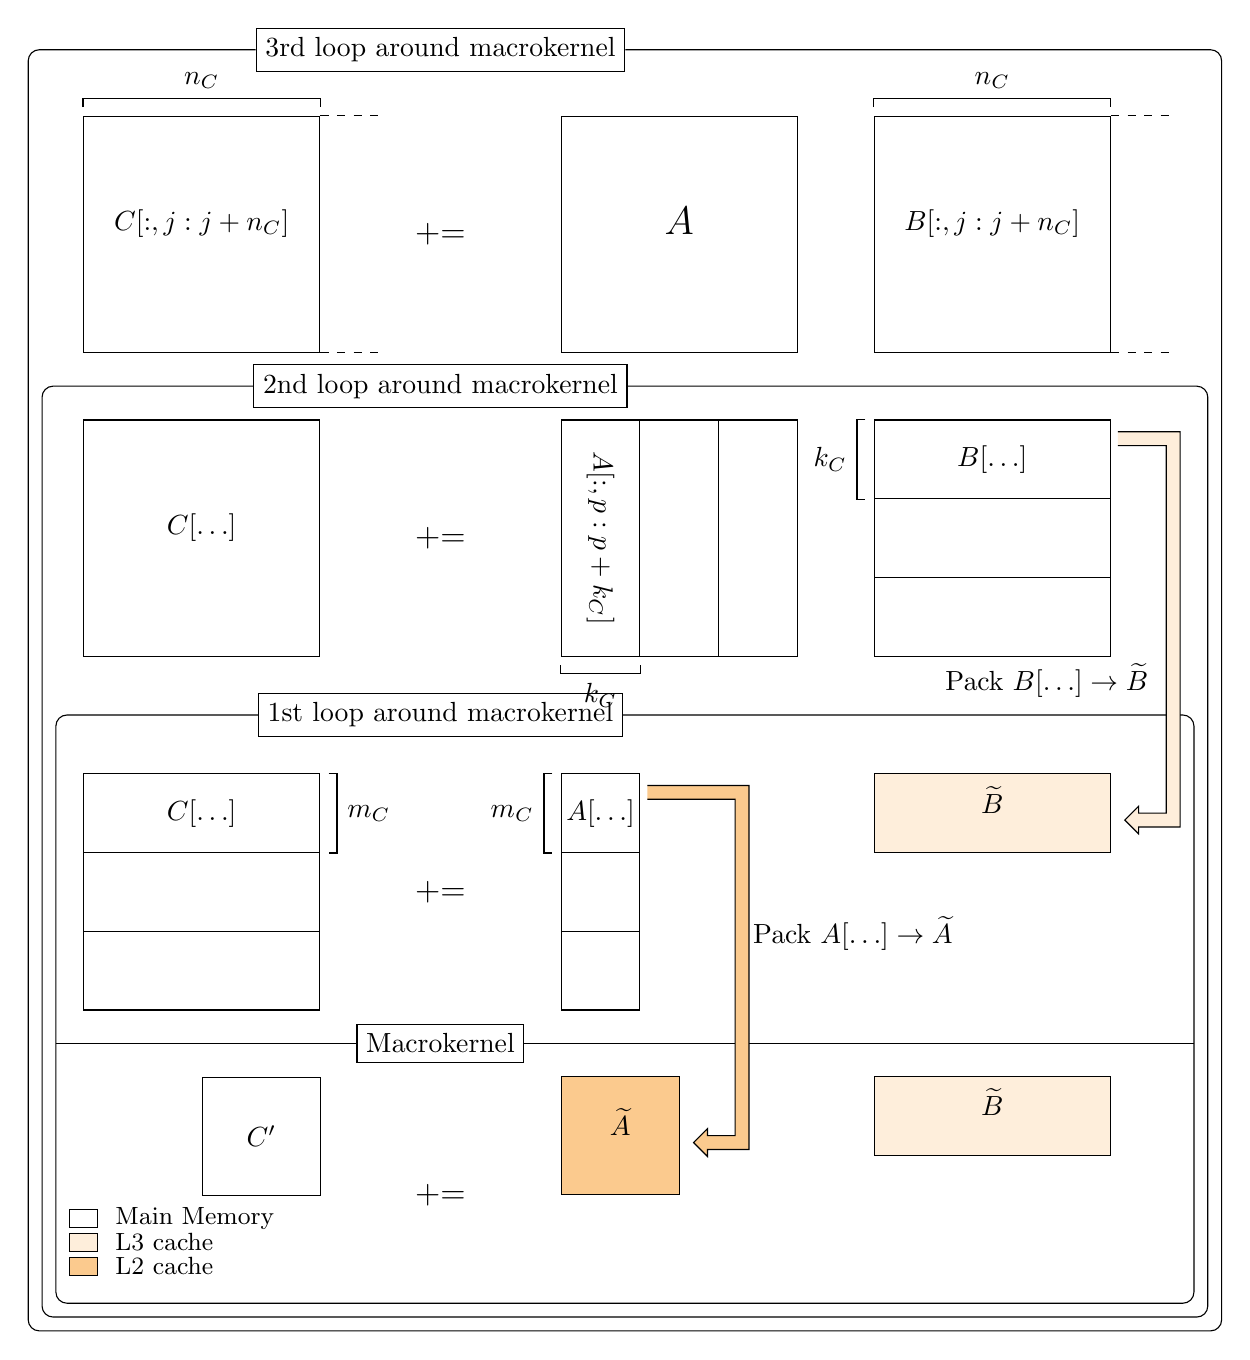
\begin{tikzpicture}
    \matrix (loops)[column sep=0.2cm, row sep=5.5ex] {
  \node[square-mat] (3C) {$C[:,j:j+n_C]$};
  \bracelabel{3C.north west}{3C.north east}{above}{$n_C$}
  \draw[dashed] (3C.north east) -- ++(0.75, 0)
  (3C.south east) -- ++(0.75, 0);&

  \pluseqnode{3}&

  \node[square-mat,memory] (3A) {\Large $A$};&

  \node[square-mat,memory] (3B) {$B[:,j:j+n_C]$};
  \bracelabel{3B.north west}{3B.north east}{above}{$n_C$}
  \draw[dashed] (3B.north east) -- ++(0.75, 0)
  (3B.south east) -- ++(0.75, 0);\\


  \node[square-mat,memory] (2C) {$C[\ldots]$};&

  \pluseqnode{2}&

  \vgrids[memory]{2A}{1}{3}{3}{}
  \node[at=(2A1),rotate=-90] {$A[:,p:p+k_C]$};
  \bracelabel{2A1.south west}{2A1.south east}{below}{$k_C$}&

  \hgrids[memory]{2B}{3}{1}{3}{}
  \node[at=(2B1)] {$B[\ldots]$};
  \bracelabel{2B1.north west}{2B1.south west}{left}{$k_C$}\\


  \hgrids[memory]{1C}{3}{1}{3}{}
  \node[at=(1C1)] {$C[\ldots]$};
  \bracelabel{1C1.north east}{1C1.south east}{right}{$m_C$}&

  \pluseqnode{1}&

  \hgrids[memory]{1A}{1}{1}{3}{}
  \node[at=(1A1)] {$A[\ldots]$};
  \bracelabel{1A1.north west}{1A1.south west}{left}{$m_C$}&

  \node[l3,wide-mat] (1B) {$\widetilde{B}$};\\

  \node[rectangle,draw,memory,at={(1.5, 0)},anchor=north west,minimum height=1.5cm, minimum width=1.5cm] (0C) {$C'$};
  \begin{scoped}[start chain=labels going {below=2pt of \tikzchainprevious}]
    \node[legend=Main Memory, memory] at (0, -1.8) {};
    \node[legend=L3 cache, l3] {};
    \node[legend=L2 cache, l2] (legend-anchor) {};
  \end{scoped}&

  \pluseqnode{0}&

  \node[l2,tall-mat,fit={(0, 0) (1.5, -1.5)}] (0A) {$\widetilde{A}$};&

  \node[l3,wide-mat,  wide-mat/.style={rectangle,draw,fit={(0, 0) (3, -1.5)},inner sep=0},] (0B) {$\widetilde{B}$};\\
};
\path node[draw,above=1.8cm of 3-plus] (3-loop){3rd loop around macrokernel}
(3-plus) -- (2-plus) node[loop-label] (2-loop){2nd loop around macrokernel}
(2-plus) -- (1-plus) node[loop-label] (1-loop) {1st loop around macrokernel}
(1-plus) -- (0-plus) node[loop-label] (0-loop) {Macrokernel};

\draw[rounded corners] let \p1 = ($(labels-end.south) + (0pt, -10pt)$),
\p2 = ($(0B.south east) + (30pt, 0)$),
\p3 = ($(labels-end.south west) + (-5pt, 0)$),
\p{east} = (\x2, \y1), \p{west} = (\x3, \y1) in
(1-loop.west) -| (\p{west}) coordinate (1-rect-west)
-- (\p{east}) coordinate (1-rect-east)
|- (1-loop.east);

\loopborder{2}{1}
\loopborder{3}{2}

\draw let \p1 = (0-loop),
\p2 = (1-rect-west),
\p3 = (1-rect-east),
\p{west-end} = (\x2, \y1),
\p{east-end} = (\x3, \y1) in
(0-loop.east) -- (\p{east-end})
(0-loop.west) -- (\p{west-end});

\path[draw, l3] (2B1.east) ++(2.5pt, 5pt) coordinate (B-arr-start)
-| ($(1B.east) + (20pt, 0pt)$) node[pos=0.82,left=3pt] {Pack $B[\ldots] \to \widetilde{B}$} coordinate (B-arr-down)
-- ++ (-10pt, 0)
-- ++(0pt, 2.5pt) -- ++(-5pt, -5pt) -- ++(5pt, -5pt) -- ++(0, 2.5pt)
-- ($(B-arr-down) + (5pt, -5pt)$)
|- ($(B-arr-start) + (0pt, 5pt)$);

\path[draw, l2] (1A1.east) ++(2.5pt, 5pt) coordinate (A-arr-start)
-| ($(0A.east) + (20pt, 0pt)$) node[pos=0.7,right=3pt] {Pack $A[\ldots] \to \widetilde{A}$} coordinate (A-arr-down)
-- ++ (-10pt, 0)
-- ++(0pt, 2.5pt) -- ++(-5pt, -5pt) -- ++(5pt, -5pt) -- ++(0, 2.5pt)
-- ($(A-arr-down) + (5pt, -5pt)$)
|- ($(A-arr-start) + (0pt, 5pt)$);

  \end{tikzpicture}
  \end{adjustbox}
\end{frame}


\begin{frame}
  \frametitle{Data reuse}
  \begin{itemize}
  \item Every loop reads \emph{something} repeatedly
  \item Relevant things: packed blocks --- making them takes time
  \item Packed block reuse problems:
    \begin{itemize}
    \item $m$ small --- low time between remakes of $\widetilde{B}$
    \item $n$ small --- same for $\widetilde{A}$
    \item $k$ tiny --- microkernel doesn't do much, small caches
    \end{itemize}
  \end{itemize}
\end{frame}

\section[\gemmt{}]{The \gemmt{} algorithm}
\frame{\sectionpage}

\begin{frame}
  \frametitle{Key concept of the algorithm}
  \begin{itemize}
  \item We want $G \pluseq DEF$, (dimensions: $m, k, l, n$ in order)
  \item $EF$ first needed in packing step
  \item Compute a block then
  \end{itemize}
\end{frame}

\begin{frame}
  \frametitle{Deriving \gemmt{}: Partitionings}
  \begin{adjustbox}{max size={!}{0.87\textheight},center}
  \begin{tikzpicture}
    \matrix (pics)[column sep=0.2cm, row sep=5.5ex, ampersand replacement=\&] {
      \&
      \node[at={(1.5, 0)}] {\large $G$};\&
      \node[at={(0, 0)}] {\large $\pluseq$};\&
      \node[at={(1.5, 0)}] {\large $D$};\&
      \node[at={(1.5, 0)}] {\large $[(EF)$};\&
      \node[at={(0, 0)}] {\large $\leftrightarrow$};\&
      \node[at={(1.5, 0)}] {\large $E$};\&
      \node[at={(1.5, 0)}] {\large $F]$};\\

      \node[at={(0, -1.5)}] {\large 1.};\&
      \node[square-mat] (2G) {\large $m \times n$};\&
      \pluseqnode{2}\&
      \node[square-mat] (2D) {\large $m \times k$};\&
      \node[square-mat, dotted] (2EF) {\large $k \times n$};
      \bracelabel{2EF.north west}{2EF.south west}{left}{}\&
      \node[at={(0, -1.5)}] {\large $\leftrightarrow$};\&
      \node[square-mat] (2E) {\large $k \times l$};\&
      \node[square-mat] (2F) {\large $l \times n$};
      \bracelabel{2F.north east}{2F.south east}{right}{}\\

      \node[at={(0, -1.5)}] {\large 2.};\&
      \node[square-mat] (1G) {\large $m \times n_C$};\&
      \pluseqnode{1}\&
      \node[square-mat] (1D) {\large $m \times k$};\&
      \node[square-mat, dotted] (1EF) {\large $k \times n_C$};
      \bracelabel{1EF.north west}{1EF.south west}{left}{}\&
      \node[at={(0, -1.5)}] {\large $\leftrightarrow$};\&
      \node[square-mat] (1E) {\large $k \times l$};\&
      \node[square-mat] (1F) {\large $l \times n_C$};
      \bracelabel{1F.north east}{1F.south east}{right}{}\\

      \node[at={(0, -1.5)}] {\large 3.};\&
      \node[square-mat] (0G) {\large $m \times n_C$};\&
      \pluseqnode{0}\&
      \node[tall-mat] (0D) {\large $m \times k_C$};\&
      \node[wide-mat, dotted] (0EF) {\large $k_C \times n_C$};
      \bracelabel{0EF.north west}{$(0, -3)$}{left}{}\&
      \node[at={(0, -1.5)}] {\large $\leftrightarrow$};\&
      \node[wide-mat] (0E) {\large $k_C \times l$};\&
      \node[square-mat] (0F) {\large $l \times n_C$};
      \bracelabel{0F.north east}{0F.south east}{right}{}\\
    };
  \end{tikzpicture}
  \end{adjustbox}
\end{frame}

\begin{frame}
  \frametitle{Deriving \gemmt{}: Inner algorithm}
  \begin{adjustbox}{max size={!}{0.5\textheight},center}
  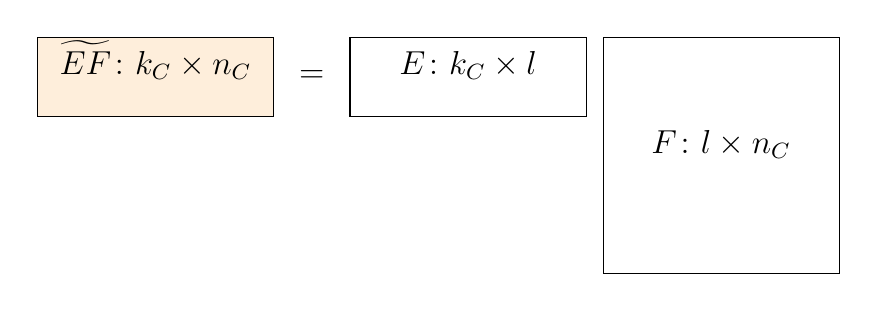
\begin{tikzpicture}
    \matrix (pics)[column sep=0.2cm, row sep=5.5ex, ampersand replacement=\&] {
      \node[wide-mat, l3] (0EF) {\large $\widetilde{EF} \colon k_C \times n_C$};\&
      \node[at={(0, -0.5)}] {\large $=$};\&
      \node[wide-mat] (0E) {\large $E \colon k_C \times l$};\&
      \node[square-mat] (0F) {\large $F \colon l \times n_C$};\\
    };
  \end{tikzpicture}
  \end{adjustbox}
  \begin{itemize}
  \item Only point to compute $EF$ in constant memory
  \item \gemm{} algorithm needs tweaks
  \end{itemize}

\end{frame}

\begin{frame}
  \frametitle{Deriving \gemmt{}: The tricky bits}
  \begin{table}
    \centering
    \begin{tabular}{l|l}
      Problem&Solution\\ \hline \hline
      Redundant loop over $n$ ($n \leq n_C$) & Remove it\\
      Packing output wastes space/time & Tweak microkernel params\\
      $\widetilde{F}$ fights $\widetilde{EF}$ in $L3$ & Halve $n_C$\\
      Low $\widetilde{F}$ reuse & Low impact in practice\\
      $m_R \nmid k_C$, leaving fringe & Shrink $k_C$ slightly\\
    \end{tabular}
    \caption{Tweaks needed to make \gemm{} fusion work}
    \label{tab:gemm3-issues}
  \end{table}
\end{frame}

\begin{frame}
  \frametitle{The algorithm}
  \begin{figure}
    \centering
    \includegraphics[height=0.875\textheight]{gemm3-picture}
    \caption{Illustration of the \gemmt{} algorithm}
    \label{fig:gemm3}
\end{figure}
\end{frame}

\begin{frame}
  \frametitle{$G \pluseq (DE)F$}
  \begin{itemize}
  \item Putting parentheses there sometimes better
  \item Deriving directly doesn't work --- bad shape
  \item However, $G \pluseq (DE)F \Leftrightarrow G^T \pluseq F^T(E^TD^T)$
  \end{itemize}
\end{frame}

\section[Results]{Experiments and Results}
\frame{\sectionpage}

\begin{frame}
  \frametitle{Implementation details}
  \begin{columns}
    \begin{column}{0.5\textwidth}
      \begin{itemize}
      \item Multilevel Optimization of Matrix Multiply Sandbox (MOMMS)
      \item Extended to support three matrices
      \item Implement both \gemmt{} and BLIS algorithm
      \item BLIS algorithm port performs like BLIS
      \item Experiments on Haswell machine from UT lab
      \end{itemize}
    \end{column}
    \begin{column}{0.5\textwidth}
      \begin{table}
        \centering
        \begin{tabular}{l|c c}
          &\gemmt{}&BLIS algorithm\\ \hline
          $m_C$&72&72\\
          $k_C$&252&256\\
          $l_C$&256&\\
          $n_C$&2040&4080\\
        \end{tabular}
        \caption{Parameters for Haswell CPUs}
        \label{tab:haswell-paramss}
      \end{table}
    \end{column}
  \end{columns}
\end{frame}

\begin{frame}
  \frametitle{Experiments}
  \begin{enumerate}
  \item $G \pluseq D(EF)$, square matrices
    \begin{itemize}
    \item Inputs column-major, outputs row-major for fairness
    \end{itemize}
  \item $G^T \pluseq F^T(E^TD^T)$, square matrices
    \begin{itemize}
    \item After transpose, all row major
    \end{itemize}
  \item $G \pluseq D(EF)$, rectangles (one dimension small)
  \end{enumerate}
\end{frame}

\begin{frame}
  \frametitle{Workspace usage, square matrices}
  \begin{tikzpicture}
    \node[graph-pic] (graph) {\includegraphics[height=0.9\textheight]{../results/earwig2/gemm3_memory}};
  \end{tikzpicture}
\end{frame}

\begin{frame}
  \frametitle{$G \pluseq D(EF)$, square matrices}
  \begin{tikzpicture}
    \node[graph-pic] (graph) {\includegraphics[height=0.9\textheight]{../results/earwig2/gemm3}};
    \node[explanation, right=1.5cm of graph.west] {\small Less packing};
    \node[explanation, below left=1.6cm and 3pt of graph.north,anchor=north] {\small Suboptimal shape};
    \node[explanation, below left=2cm and 1cm of graph.north east, anchor=east] {\small Memop overhead};
  \end{tikzpicture}
\end{frame}

\begin{frame}
  \frametitle{$G \pluseq (DE)F$, square matrices}
  \begin{tikzpicture}
    \node[graph-pic] (graph) {\includegraphics[height=0.9\textheight]{../results/earwig2/gemm3_ab_bc_kernel}};
    \node[explanation, at=(graph.center)] {\small Similar trends, row-major helps BLIS};
  \end{tikzpicture}
\end{frame}

\begin{frame}
  \frametitle{$G \pluseq D(EF)$, rectangular matrices}
  \begin{tikzpicture}
    \node[graph-pic] (graph) {\includegraphics[height=0.9\textheight]{../results/earwig2/gemm3_rectangles}};
  \end{tikzpicture}
\end{frame}

\section{Conclusions}
\begin{frame}
  \frametitle{Conclusions}
  \begin{itemize}
  \item \gemm{} structure lets us make \gemmt{}
  \item Constant memory
  \item Comprable performance
  \item Cleaner API
  \end{itemize}
\end{frame}

\begin{frame}
  \frametitle{Future Work}
  \begin{itemize}
  \item Parallel case
  \item More architectures
  \end{itemize}
\end{frame}

\begin{frame}
  \frametitle{Acknowledgments}
  \begin{itemize}
  \item Prof.\ Robert van de Geijn --- advising and providing inspiration
  \item Dr.\ Tyler Smith --- writing MOMMS and algorithm design
  \item Prof.\ Tze Meng Low --- performance fixes
  \item NSF grant \textbf{TODO NNNNNNN} --- funding
  \end{itemize}
\end{frame}

\begin{frame}
  \frametitle{Questions?}
\end{frame}

\section{Picking parameters}
\begin{frame}
  \frametitle{Picking parameters: $m_R, n_R$}
  \begin{itemize}
  \item Determine microkernel
  \item Based on microarchitecture --- register width, FMA properties
  \item We're reusing BLIS's work
  \item Can swap $m_R$ and $n_R$
  \end{itemize}
\end{frame}

\begin{frame}
  \frametitle{Picking parameters: $k_C$}
  Placing memory in cache: [tag][set \#][offset in line]

  \begin{equation*}
    m_rk_cS_{elem} = C_AC_{L1}N_{L1} \qquad n_rk_CS_{elem} = C_BC_{L1}N_{L1}
  \end{equation*}

  \begin{columns}
    \begin{column}{0.1\textwidth}
      L1 Cache:
    \end{column}
    \begin{column}{0.5\textwidth}
      \centering
      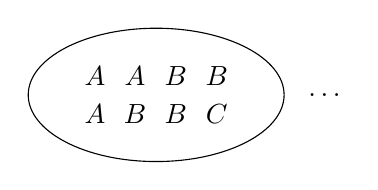
\begin{tikzpicture}
        \matrix (labels) [matrix of math nodes, ampersand replacement=\&] {
          A \& A \& B \& B\\
          A \& B \& B \& C\\
        };
        \node[draw, ellipse, fit={(labels-1-1) (labels-2-4)}] (labels-border) {};
        \node[right=5pt of labels-border] {$\ldots$};
      \end{tikzpicture}
    \end{column}
    \begin{column}{0.25\textwidth}
      \begin{equation*}
        C_A + C_B + 1 \leq W_{L1}
      \end{equation*}
    \end{column}
  \end{columns}
  \begin{center}
    Maximizing $k_C$ improves performance
  \end{center}

  \begin{align*}
    C_B &= \ceil*{\frac{n_Rk_CS_{elem}}{N_{L1}C_{L1}}}\\
        &= \ceil*{\frac{n_R}{m_R}C_A}\\
    C_A &\leq \floor*{\frac{W_{L1} - 1}{1 + \frac{n_R}{m_R}}}
  \end{align*}
\end{frame}

\begin{frame}
  \frametitle{Picking parameters: $m_C$ and $n_C$}
  \begin{itemize}
  \item For $m_C$: reserve ways for $B$ and $C$
  \item Then take all you can
  \item $n_C$, leave out what architecture requires, then divide
  \item L3 is very big, tuning is much less needed
  \end{itemize}
\end{frame}
\end{document}
